\subsection{Profile screens}\label{subsec:profile-screens}
\textbf{Profile screen} (Figure \ref{fig:profile}) represents the menu of the application.
A user has granted access to his profile, management block, and he can see the set default aircraft and device.
In addition, if he belongs to an organization, it shows him the organization name and the button to switch the fleet mode.
My management container contains My Flights, My Devices and My Aircrafts buttons.

\textbf{Profile detail} contains the user properties like the full name, phone number and country.
In addition, it allows changing the user contact e-mail and password.


\begin{figure}
    \centering
    \begin{minipage}{.45\textwidth}
        \centering
        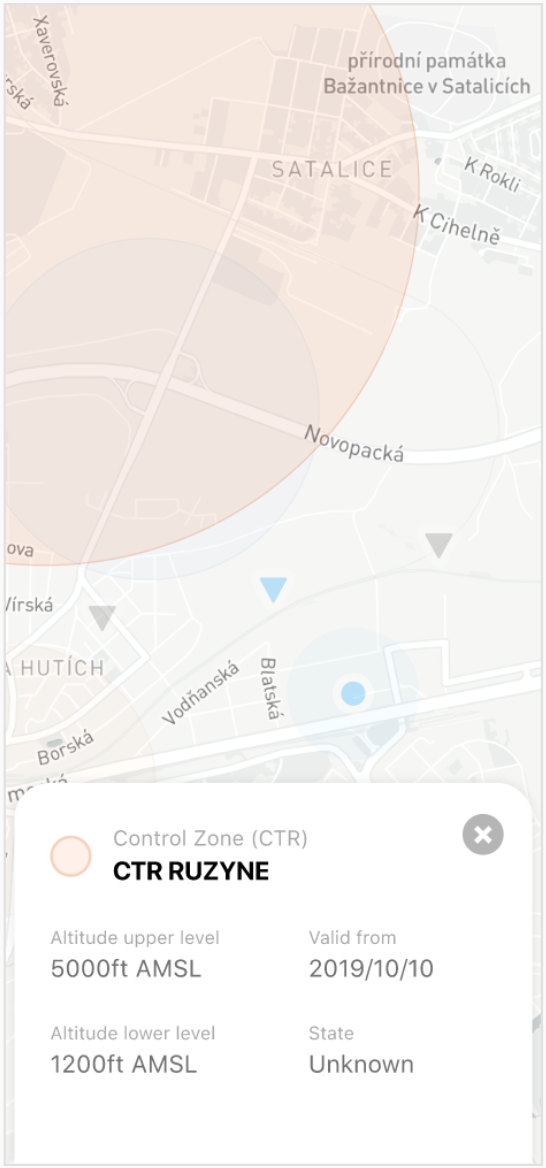
\includegraphics[width=.7\linewidth]{assets/user_interface_design/dashboard/dashboard_zone_detail.png}
        \caption{[A70] Dashboard, Zone detail}
        \label{fig:dashboard_zone_detail}
    \end{minipage}%
    \hspace{.05\linewidth}
    \begin{minipage}{.45\textwidth}
        \centering
        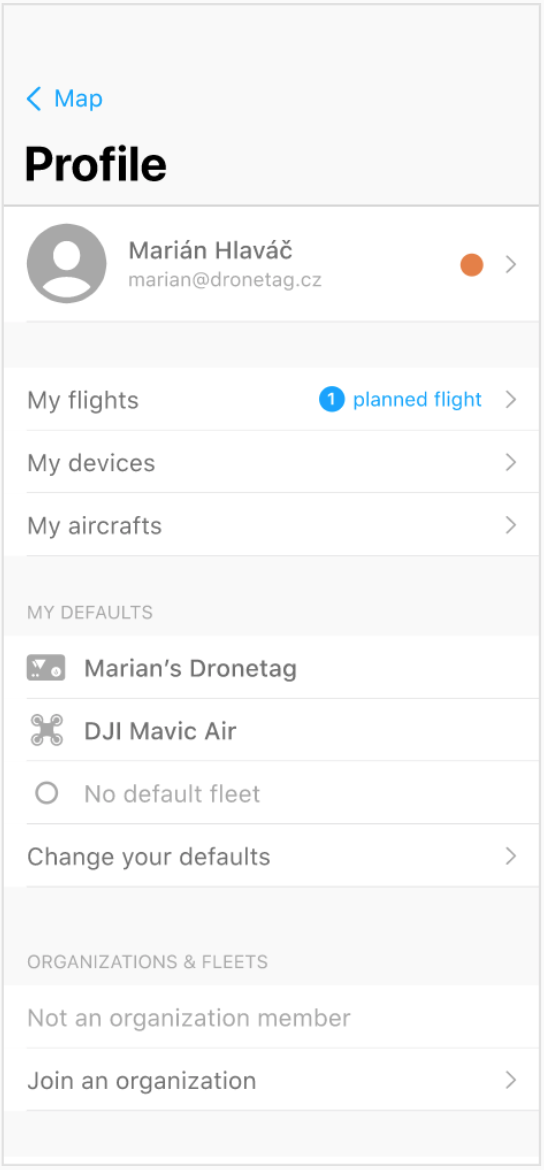
\includegraphics[width=.7\linewidth]{assets/user_interface_design/profile/profile.png}
        \caption{[A13] Profile}
        \label{fig:profile}
    \end{minipage}
    \label{fig:profile_all}
\end{figure}
